%%%%%%%%%%%%%%%%%%%%%%%%%%%%%%%%%%%%%%%%%%%%%%%%%%%%%%%%%%%%%%%%%%%%%%%%%%%%%%%%%%%%%%%%%%%%%%%%%%%%%%%%%%%%%%%%%
%% Kapitel 2 - Stand der Forschung und Technik %%%%%%%%%%%%%%%%%%%%%%%%%%%%%%%%%%%%%%%%%%%%%%%%%%%%%%%%%%%%%%%%%%
%%%%%%%%%%%%%%%%%%%%%%%%%%%%%%%%%%%%%%%%%%%%%%%%%%%%%%%%%%%%%%%%%%%%%%%%%%%%%%%%%%%%%%%%%%%%%%%%%%%%%%%%%%%%%%%%%
\chapter{Stand der Forschung und Technik} \label{chap:stand}

Dieses Kapitel stellt die für diese Arbeit erforderlichen technischen und methodischen Grundlagen bereit. Zunächst werde in Abschnitt~\ref{sec:zuv} zentrale Begriffe und Konzepte der Zuverlässigkeitstechnik sowie das grundlegende statistische Verfahren zur Lebensdauer-Datenanalyse in Kombination mit Versuchsplänen erläutert.
Darauf aufbauend folgen in Abschnitt~\ref{sec:doe} die Einführung und die Einordnung von \acs{DoE} sowie der multivariaten Lebensdauermodellierung aus dem Stand der Technik und der Wissenschaft, die beide für die Entwicklung effizienter Lebensdauerversuchspläne maßgeblich sind.
Im Kontext der Lebensdauererprobung umfasst dies insbesondere typische, statistische Versuchspläne sowie Metriken und Indikatoren zur allgemeinen Bewertung der Versuchspläne.

\section{Zuverlässigkeitstechnik und Wahrscheinlichkeitstheorie} \label{sec:zuv}
Die Zuverlässigkeitstechnik befasst sich mit der probabilistischen Beschreibung der Lebensdauer technischer Produkte und Systeme sowie der strategischen und statistischen Planung von Lebensdauertests.
Ziel ist die statistische Modellierung des Ausfallverhaltens unter Berücksichtigung der Funktionalität des Produkts bei relevanten Randbedingungen.
Eine zentrale Aufgabe besteht somit in der statistischen Charakterisierung des Ausfallbegriffs mithilfe deskriptiver Statistik sowie in der Parametrisierung geeigneter Verteilungen zur Abbildung des Lebensdauerverhaltens.
Die Modellierung kann - abhängig von den Randbedingungen - auf Basis \textit{einer einzelnen} Belastungsgröße oder \textit{mehrerer} Beanspruchungsparameter erfolgen, die gemeinsam den Produktausfall determinieren.
Ein grundlegendes Verständnis des Umgangs mit zufallsverteilten Lebensdauerereignissen ist daher eine elementare Voraussetzung für die statistische Versuchsplanung im Rahmen der Zuverlässigkeitstechnik.
Weiterführende Konzepte und vertiefte methodische Ansätze zur Zuverlässigkeitstechnik sowie zur statistischen Testplanung sind allen voran in der Standardliteratur von Bertsche und Dazer \cite{Bertsche.2022} dargelegt, an deren Vorgehensweise sich die nachfolgenden Ausführungen orientieren.

\subsection{Begriffe und Definitionen} \label{subsec:begriffezuv}
Der \textbf{Ausfall} eines technischen Produkts bezeichnet den Zeitpunkt innerhalb seiner Lebensdauer, zu dem die geforderte Funktionalität unter definierten Umgebungs- und Randbedingungen nicht mehr erfüllt ist - also das Lebensdauerende - engl. \textbf{\ac{EoL}}.
Als \textbf{Belastung} werden die von außen auf ein Produkt einwirkenden Einflussparameter - Kräfte und Momente im mechanischen Kontext - bezeichnet.
\textit{Einzelne} oder zeitgleich \textit{mehrere} Einflussparameter induzieren infolge der Produktgestalt daraus \textbf{Beanspruchungen}: innere Kräfte, Momente und lokale Spannungen.
Belastung und Beanspruchung sind die maßgeblichen Faktoren, welche die Lebensdauer determinieren.
Die \textbf{Ausfallzeit}, welche diese Zustandsänderung zeitlich definiert, wird im Allgemeinen als kontinuierliche Zufallsvariable $\sym{tau}>0$ aufgefasst.
So ergibt sich die Wahrscheinlichkeit, dass ein Produkt im Zeitraum bis $\sym{t}$ einen Funktionsverlust erleidet, zu
\begin{equation} \label{eq:probdef}
    \sym{F}(\sym{t})=\sym{Pr}(\sym{tau}\leq \sym{t}) = \int_{0}^{\sym{t}} \sym{f}(\sym{t}) \,d\sym{t}.
\end{equation}
Diese Funktion beschreibt die \textbf{Ausfallwahrscheinlichkeit}.
Sie definiert damit die Verteilungsfunktion - engl. \textbf{\ac{cdf}} - für stochastische \ac{EoL}-Events, während die \textbf{Zuverlässigkeit}
\begin{equation} \label{eq:reldef}
    \sym{R}(\sym{t})=\sym{Pr}(\sym{tau} > \sym{t}) = 1 - \sym{F}(\sym{t}) = \int_{\sym{t}}^{\infty} \sym{f}(\sym{t}) \,d\sym{t} , \quad \sym{t} \geq 0.
\end{equation}
komplementär diejenige Wahrscheinlichkeit $\sym{R}(\sym{t}): \sym{RR}_{\geq 0} \rightarrow [0,1] \subset \sym{RR}$ quantifiziert, zu der das nicht reparierbare Produkt die realisierte Zeit $\sym{t}$ überlebt: also frei von Funktionsverlust bleibt und funktionsfähig ist \cite{Bertsche.2022,Birolini.2017,Meeker.2022}.
Damit ist die Zuverlässigkeit mathematisch als reellwertige, monoton fallende und stetige Funktion definiert.
Gleichwohl ist $\sym{R}(\sym{t})$ keine universelle Eigenschaft, sondern vielmehr eine Funktion der Betriebsbedingungen .
Diese Bedingungen umfassen unter anderem eine oder mehrere Belastungsarten und deren Niveaus, Nutzungsverhalten sowie
spezifische Betriebsprofile. Mechanische, elektrische und thermische Belastungen treten dabei am häufigsten auf \cite{Yang.2007}.
Die \textbf{Wahrscheinlichkeitsdichtefunktion} - engl. \textbf{\ac{pdf}} - $\sym{f}(\sym{t})$ der Ausfallzeit beschreibt, wie sich die Wahrscheinlichkeiten der Ausfälle über der Zeit verteilen.
Sie folgt somit der Ableitung der \ac{cdf}:
\begin{equation} \label{eq:pdfdef}
    \sym{f}(\sym{t}) = \frac{d}{d\sym{t}}\sym{F}(\sym{t}) = \frac{d}{d\sym{t}}\sym{Pr}(\sym{tau} \leq \sym{t}), \quad \sym{t} \geq 0.
\end{equation}
Damit repräsentiert $\sym{f}(\sym{t})$ die Ausfallintensität pro Zeiteinheit und ist proportional zur lokalen Änderungsrate der Ausfallwahrscheinlichkeit.
Als vierte fundamentale Größe der Zuverlässigkeitsanalyse wird außerdem die \textbf{Ausfallrate} (auch Hazard-Funktion) $\sym{lambda}(\sym{t})$ eingeführt.
Sie quantifiziert das momentane Ausfallrisiko eines Produkts zum Zeitpunkt $\sym{t}$, bedingt dadurch, dass es bis zu diesem Zeitpunkt überlebt hat ($\sym{R}(\sym{t}) > 0$).
Mathematisch ist sie als das Verhältnis der \ac{pdf} zur Zuverlässigkeitsfunktion $\sym{R}(\sym{t})$ definiert:
\begin{equation} \label{eq:hazarddef}
    \sym{lambda}(\sym{t}) = \lim_{\Delta \sym{t} \to 0} \frac{\sym{Pr}(\sym{t} < \sym{tau} \leq \sym{t} + \Delta \sym{t} | \sym{tau} > \sym{t})}{\Delta \sym{t}} = \frac{1}{\sym{R}(\sym{t})} \left[ - \frac{d\sym{R}(\sym{t})}{d\sym{t}} \right] = \frac{\sym{f}(\sym{t})}{\sym{R}(\sym{t})} .
\end{equation}
Die Ausfallrate $\sym{lambda}(\sym{t})$ ist von zentraler Bedeutung, da ihr zeitlicher Verlauf (z.B. konstant, steigend, fallend) direkte Rückschlüsse auf zugrundeliegende Ausfallmechanismen wie Frühausfälle, Zufallsausfälle oder Verschleiß (vgl. "Badewannenkurve") zulässt \cite{Bertsche.2022,Yang.2007,Rigdon.2022}.

\subsection{Deskriptive Statistik für Lebensdauerdaten} \label{subsec:stat}
Die im vorherigen Abschnitt definierten Funktionen $\sym{F}(\sym{t})$, $\sym{R}(\sym{t})$, $\sym{f}(\sym{t})$ und $\sym{lambda}(\sym{t})$ beschreiben das stochastische Ausfallverhalten eines Produktes auf einer theoretischen Populationsebene.
Für die praktische Anwendung im Engineering müssen diese Funktionen, respektive die Parameter der ihnen zugrundeliegenden Verteilungsmodelle, auf Basis von empirisch ermittelten Lebensdauerdaten jedoch approximiert werden.

Die deskriptive Statistik stellt die notwendigen Methoden zur initialen Charakterisierung, Quantifizierung und Aufbereitung dieser Stichprobendaten bereit.
Zur Beschreibung der Lebensdauerverteilungen sind \textbf{Lageparameter} und \textbf{Streuungsmaße} notwendig, die zunächst theoretisch (für die Grundgesamtheit) definiert und anschließend aus der Stichprobe berechnet werden.

Der primäre Lageparameter ist der \textbf{Erwartungswert} $\sym{mu}$ der Zufallsvariable $\sym{tau}$.
Er repräsentiert den Schwerpunkt von $\sym{f}(\sym{t})$ und wird für kontinuierliche Lebensdauerdaten berechnet als:
\begin{equation} \label{eq:theo_mean}
    \sym{mu} = \sym{E}[\sym{tau}] = \int_{0}^{\infty} \sym{t} \cdot \sym{f}(\sym{t}) d\sym{t}.
\end{equation}
Ein weiterer Lageparameter ist das \textbf{Quantil} $\symsub{t}{q}$ der Lebensdauer.
Es definiert den Zeitpunkt, zu dem $\sym{F}(\sym{t})$ den Anteil $\sym{q}$ (respektive das \textbf{Perzentil} in Prozentpunkten) erreicht:
\begin{equation} \label{eq:quantildef}
    \sym{F}(\symsub{t}{q}) = \sym{q}, \quad \sym{q} \in [0,1].
\end{equation}
Damit gibt das $\sym{q}$~-~Quantil denjenigen Lebensdauerwert an, unterhalb dessen der Anteil $\sym{q}$ aller betrachteten Produkte ausgefallen ist.
Ein spezieller Fall ist der \textbf{Median} $\sym{t}_{0.5}$, bei dem die Ausfallwahrscheinlichkeit 50\% beträgt:
\begin{equation} \label{eq:mediandef}
    \sym{F}(\sym{t}_{0.5}) = 0.5.
\end{equation}
Der Median beschreibt somit den Zeitpunkt, zu dem die Hälfte aller Produkte ausgefallen ist.
Damit teilt er die Fläche 1 unter der \ac{pdf} in zwei gleich große Teilflächen \cite{Yang.2007,Fahrmeir.2016}.

Das primäre Streuungsmaß ist die \textbf{theoretische Varianz} $\sym{sigma_sq}$, welche die mittlere quadratische Abweichung vom Erwartungswert beschreibt:
\begin{equation} \label{eq:theo_variance}
    \sym{sigma_sq} = \sym{Var}[\sym{tau}] = \sym{E}[(\sym{tau} - \sym{mu})^2] = \int_{0}^{\infty} (\sym{t} - \sym{mu})^2 \cdot \sym{f}(\sym{t}) d\sym{t}.
\end{equation}
Da $\sym{mu}$ und $\sym{sigma_sq}$ als theoretische Parameter üblicherweise unbekannt sind, werden auch sie durch empirische Statistiken approximiert, die aus einer Stichprobe vom Umfang $\sym{n}$ (bestehend aus den Messwerten $\sym{x}_{1}, \dots, \symsub{x}{n}$) berechnet werden.
Diese werden wiederum als Realisierungen der Zufallsvariable $\sym{tau}$ aufgefasst.

Das gängige empirische Äquivalent für den Erwartungswert $\sym{mu}$ ist der \textbf{arithmetische Mittelwert} $\sym{x_bar}$:
\begin{equation} \label{eq:emp_mean}
    \sym{x_bar} = \frac{1}{\sym{n}} \sum_{\sym{i}=1}^{\sym{n}} \symsub{x}{i}.
\end{equation}
Analog wird die theoretische Varianz $\sym{sigma_sq}$ durch die \textbf{empirische Varianz} $\sym{s_sq}$ (eine erwartungstreue Kenngröße) approximiert:
\begin{equation} \label{eq:emp_variance}
    \sym{s_sq} = \frac{1}{\sym{n}-1} \sum_{\sym{i}=1}^{\sym{n}} (\symsub{x}{i} - \sym{x_bar})^2.
\end{equation}
Die \textbf{empirische Standardabweichung} $\sym{s} = \sqrt{\sym{s_sq}}$ dient entsprechend als Näherung für die theoretische Standardabweichung $\sqrt{\sym{sigma_sq}}$.\

\subsection{Parametrische Lebensdauermodelle} \label{subsec:paramleben}

Während die deskriptiven Statistiken $\sym{x_bar}$ und $\sym{s_sq}$ die zentrale Tendenz und die Streuung der vorliegenden Stichprobe quantifizieren, erlauben sie keine Extrapolation oder die Modellierung der zugrundeliegenden Funktionen $\sym{F}(\sym{t})$ und $\sym{f}(\sym{t})$ der Grundgesamtheit.
Um eine prädiktive, mathematische Beschreibung des stochastischen Ausfallverhaltens zu erhalten, müssen die in Abschnitt~\ref{subsec:begriffezuv} definierten Lebensdauerfunktionen durch geeignete parametrische Verteilungsmodelle approximiert werden.
Diese Verteilungsmodelle bieten eine geschlossene mathematische Form für \ac{cdf} und \ac{pdf} und ermöglichen es, das komplexe Ausfallverhalten durch eine geringe Anzahl von Parametern zu charakterisieren.\

\subsubsection{Weibull-Verteilung} \label{subsubsec:weibull}
In der Zuverlässigkeitstechnik hat sich die \textbf{Weibull-Verteilung} aufgrund ihrer hohen Flexibilität als das am häufigsten verwendete Modell etabliert.
Je nach zugrundeliegendem physikalischen Ausfallmechanismus finden jedoch auch andere statistische Verteilungen Anwendung, wie beispielsweise die \textbf{Lognormal-Verteilung} (häufig bei Ermüdungs-, Korrosions- oder Diffusionsprozessen), die \textbf{Exponentialverteilung} (zur Modellierung von Zufallsausfällen ohne Alterungseffekte) oder die \textbf{Beta-Verteilung} (allgemein zur formenreichen Modellierung von $\sym{R}$ über dem festen Intervall $[0,1]$).
Für weitere Ausführungen dazu sei an dieser Stelle jedoch auf bereits ausreichend diskutierte Beiträge in beispielsweise  \cite{Bertsche.2022,Yang.2007,Birolini.2017,Hedderich.2020} verwiesen.

Die (zwei-parametrige) Weibull-Verteilung ist das Standardmodell zur Beschreibung der Lebensdauer von technischen Produkten ohne die Berücksichtigung eines möglichen dritten Parameters - der ausfallfreien Zeit \symsub{t}{0}.
Sie wird durch den \textbf{Formparameter}  $\sym{b} > 0$ (Weibull-Modul) und die \textbf{charakteristische Lebensdauer} $\sym{T} > 0$ (Skalenparameter), welche dem $63,2$-ten Perzentil $\sym{t}_{0,632}$ entspricht, beschrieben.
Unabhängig von $\sym{b}$ gilt hier: $\sym{F}(\sym{T})=1-e^{-1} \approx 63,2 \%$.
Folgt die Lebensdauer-Zufallsvariable $\sym{tau}$ dieser Verteilung, wird dies mathematisch als $\sym{tau} \sim \sym{W}(\sym{T}, \sym{b})$ notiert.
Damit ist sie in der Lage, alle drei Phasen der "Badewannenkurve" (Frühausfälle mit $\sym{b}<1$, Zufallsausfälle $\sym{b}\approx 1$, Verschleißausfälle mit $\sym{b}>1$) durch die Wahl ihrer Parametrisierung abzubilden, vgl. \cite{Bertsche.2022}.

Die Einheit des Skalenparameters $\sym{T}$ entspricht der Einheit des Messwertes ($\sym{t}$ in Stunden, Überrollungen, Kilometer, etc.).
Die \ac{pdf} der Weibull-Verteilung ist damit definiert als:
\begin{equation} \label{eq:weibull_pdf}
    \sym{f}(\sym{t}) = \frac{\sym{b}}{\sym{T}^{\sym{b}}} \sym{t}^{\sym{b}-1} \exp\left[ - \left(\frac{\sym{t}}{\sym{T}}\right)^{\sym{b}} \right], \quad \sym{t} > 0.
\end{equation}
Die \ac{cdf} ergibt sich durch Integration der \ac{pdf} zu:
\begin{equation} \label{eq:weibull_cdf}
    \sym{F}(\sym{t}) = 1 - \exp\left[ - \left(\frac{\sym{t}}{\sym{T}}\right)^{\sym{b}} \right], \quad \sym{t} > 0.
\end{equation}
Aus $\sym{f}(\sym{t})$ und $\sym{R}(\sym{t}) = 1 - \sym{F}(\sym{t})$ leitet sich die \textbf{Ausfallrate} $\sym{lambda}(\sym{t})$ der Weibull-Verteilung ab:
\begin{equation} \label{eq:weibull_hazard}
    \sym{lambda}(\sym{t}) = \frac{\sym{b}}{\sym{T}} \left(\frac{\sym{t}}{\sym{T}}\right)^{\sym{b}-1}, \quad \sym{t} > 0.
\end{equation}
Der Erwartungswert $\sym{mu}$ (vgl. Gleichung~\eqref{eq:theo_mean}) und die Varianz $\sym{sigma_sq}$ (vgl. Gleichung~\eqref{eq:theo_variance}) der Weibull-Verteilung lassen sich ebenfalls in geschlossener Form ausdrücken. Sie sind von der \textbf{Gamma-Funktion} $\sym{Gamma}(\cdot)$ abhängig, welche für $x > 0$ definiert ist als:
\begin{equation} \label{eq:gamma_func}
    \sym{Gamma}(x) = \int_{0}^{\infty} \sym{z}^{x-1} \exp(-\sym{z}) \,d\sym{z}.
\end{equation}
Der Erwartungswert $\sym{mu}$ der Weibull-verteilten Lebensdauer $\sym{tau}$ ergibt sich zu:
\begin{equation} \label{eq:weibull_mean}
    \sym{mu} = \sym{E}[\sym{tau}] = \sym{T} \cdot \sym{Gamma}\left(1 + \frac{1}{\sym{b}}\right).
\end{equation}
Die Varianz $\sym{sigma_sq}$ ist gegeben durch:
\begin{equation} \label{eq:weibull_variance}
    \sym{sigma_sq} = \sym{Var}[\sym{tau}] = \sym{T}^2 \left[ \sym{Gamma}\left(1 + \frac{2}{\sym{b}}\right) - \sym{Gamma}^2\left(1 + \frac{1}{\sym{b}}\right) \right].
\end{equation}

Die Ausprägung der erwähnten Flexibilität der Weibull-Verteilung ist durch Abbildung~\ref{fig:abb2.1_weibull} nachvollziehbar.
Ein Spezialfall tritt ein für $\sym{b}=1$, da sich in diesem Fall die Weibull-Verteilung zur Exponentialverteilung mit dem Ausfallraten-Parameter $\sym{lambda} = 1/\sym{T}$ und dem Erwartungswert $\sym{mu} = \sym{T}$ reduziert.
Für $\sym{b}=3,6$ wird die Schiefe der \ac{pdf} annähernd eliminiert, sodass sich die Weibull-Verteilung einer Normalverteilung annähert \cite{Rinne.2008, Kececioglu.2002}.


\begin{figure}
    \centering
    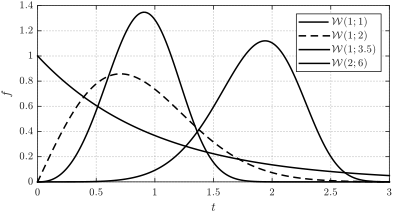
\includegraphics[width=0.9\textwidth]{plots/ma_abb2.1_weibull}
    \caption{Weibull $\sym{f}(\sym{t})$ für ausgewählte Werte von $\sym{T}$ und $\sym{b}$. }
    \label{fig:abb2.1_weibull}
\end{figure}

\subsection{Parameterschätzverfahren} \label{subsec:schätzer}
Soll eine geschlossene mathematische Beschreibung des stochastischen Ausfallverhaltens eines Produktes gefunden werden, ist das im vorherigen Abschnitten~\ref{subsec:stat} definierte parametrische Verteilungsmodell $\sym{tau} \sim \sym{W}(\sym{T}, \sym{b})$ zu schätzen.
Die Modellparameter der Grundgesamtheit sind in der praktischen Anwendung jedoch unbekannt.
Die zentrale Problemstellung der \textbf{Parameterschätzung} besteht somit darin, aus der empirischen Stichprobe bestehend aus $\sym{n}$ Realisierungen $\sym{t}_{1}, \dots, \symsub{t}{n}$ der Zufallsvariable $\sym{tau}$ statistisch fundierte Schätzwerte $\hat{\sym{T}}$ und $\hat{\sym{b}}$ zu gewinnen.
Diese sind Voraussetzung, um das Lebensdauermodell (z.B. Gleichung~\eqref{eq:weibull_cdf}) zu quantifizieren und prädiktive Aussagen zu Quantilen oder der Zuverlässigkeit $\sym{R}(\sym{t})$ zu ermöglichen.
Eine wesentliche Komplikation hierbei sind jedoch das mögliche Auftreten von unvollständigen bzw. \textbf{zensierten} Daten sowie \textit{multivariate} Abhängigkeiten der Belastungen zur Messgröße.
Während für die Schätzung von Verteilungsparametern einfache Verfahren, wie die \textbf{Momentenmethode} oder die \textbf{Methode der kleinsten Fehlerquadrate} - engl. \ac{OLS}, die beispielsweise bei der \ac{MMR} im Wahrscheinlichkeitsnetz Anwendung findet, existieren, sind diese für die umfassende Analyse vielschichtiger Lebensdauerdaten in der Regel unzureichend und hier nur der Vollständigkeit wegen erwähnt - vgl. \cite{Bertsche.2022,Montgomery.2021}.
Das universell anwendbare und robuste Verfahren, das Herausforderungen wie zensierte Daten und multivariate Modelle inhärent behandelt, ist die \ac{MLE} \cite{Bertsche.2022,Meeker.2022,Nelson.1990}.

\subsubsection{Maximum-Likelihood-Estimation} \label{subsubsec:mle}
Das Grundprinzip der \ac{MLE} besteht darin, diejenigen Parameterwerte (z.B. $\hat{\sym{T}}, \hat{\sym{b}}$) als Schätzwerte auszuwählen, welche die Wahrscheinlichkeit (engl. Likelihood) maximieren, die empirisch beobachtete Stichprobe (bestehend aus unabhängigen Ausfällen und Zensierungen) zu erhalten.
Mathematisch wird die Wahrscheinlichkeit der Realisierung von $\sym{t_vec} = (\sym{t}_{1}, \dots, \symsub{t}{n})$ einer Stichprobe durch die \textbf{Likelihood-Funktion} $\sym{L_like}$ bestimmt. Diese ist eine Funktion des unbekannten Parametervektors $\sym{theta}$, der $\sym{k}$ zu schätzende Parameter enthält (z.B. $\sym{theta} = (\sym{T}, \sym{b})$ mit $\sym{k}=2$).\

Für den vereinfachten Fall, dass die Stichprobe ausschließlich aus $\sym{n}$ exakten Ausfallereignissen (vollständige Daten) besteht, ist die Likelihood-Funktion $\sym{L_like}$ das Produkt der einzelnen Wahrscheinlichkeitsdichten $\sym{f}(\cdot)$:
\begin{equation} \label{eq:mle_likelihood_simple}
    \sym{L_like}(\sym{t_vec} | \sym{theta}) = \prod_{\sym{i}=1}^{\sym{n}} \sym{f}(\symsub{t}{i} | \sym{theta}).
\end{equation}
Zur Vereinfachung der numerischen Berechnung wird in der Anwendung die \textbf{Log-Likelihood-Funktion} $\sym{Lambda}$ verwendet. Durch die Logarithmierung wird das Produkt (Gleichung~\eqref{eq:mle_likelihood_simple}) in eine äquivalente, leichter zu maximierende Summe überführt:
\begin{equation} \label{eq:mle_loglikelihood_simple}
    \sym{Lambda} \defeq \ln\left( \sym{L_like}(\sym{theta}) \right) = \sum_{\sym{i}=1}^{\sym{n}} \ln \left[ \sym{f}(\symsub{t}{i} | \sym{theta}) \right].
\end{equation}
Wie zuvor dargelegt, ist dieser vereinfachte Ansatz für Lebensdauerdaten jedoch oft unzureichend, da er das Auftreten von zensierten Daten vernachlässigt.
Für die praktische Anwendung existiert jedoch die entsprechende Erweiterung der Likelihood-Funktion um die Differenzierung etwaiger Testausgänge als \textit{Durchläufer}.
Dazu wird die Stichprobe als Paarung von $\symsub{t}{i}, \symsub{delta}{i}$ für $\sym{t_vec}$ definiert, wobei $\symsub{t}{i}$ der beobachteten Zeit und $\symsub{delta}{i}$ einem Statusindikator ($\symsub{delta}{i}=1$ für einen exakten Ausfall; $\symsub{delta}{i}=0$ für eine Rechts-Zensierung) entspricht \cite{Bertsche.2022, Meeker.2022,Wu.2021,Yang.2007,Rigdon.2022}.
$\sym{L_like}$ für rechts-zensierte Lebensdauerdaten lautet somit:
\begin{equation} \label{eq:mle_likelihood_censored}
    \sym{L_like}(\sym{t_vec} | \sym{theta}) = \prod_{\sym{i}=1}^{\sym{n}} \left[ \sym{f}(\symsub{t}{i} | \sym{theta})^{\symsub{delta}{i}} \cdot \sym{R}(\symsub{t}{i} | \sym{theta})^{1 - \symsub{delta}{i}} \right]
\end{equation}
und definiert die Log-Likelihood Funktion als:
\begin{equation} \label{eq:mle_loglikelihood_censored}
    \sym{Lambda} \defeq \ln\left(\sym{L_like}(\sym{t_vec} | \sym{theta})\right) = \sum_{\sym{i}=1}^{\sym{n}} \left[ \symsub{delta}{i} \cdot \ln \sym{f}(\symsub{t}{i} | \sym{theta}) + (1 - \symsub{delta}{i})) \cdot \ln \sym{R}(\symsub{t}{i} | \sym{theta}) \right].
\end{equation}

Der Parametervektor $\hat{\sym{theta}}$, der den Wert von $\sym{Lambda}(\sym{theta})$ maximiert, liefert die \ac{MLE}-Werte.
Die Schätzwerte repräsentieren die (asymptotisch) effizientesten Schätzwerte für die Parameter der Grundgesamtheit.
Dies erfolgt mathematisch durch Nullsetzen $\sym{k}$ partieller Ableitungen von $\sym{Lambda}$, sofern mathematisch entsprechende Schätzwerte in geschlossener Form durch $\partial\sym{Lambda}/\partial \sym{theta} \stackrel{!}{=} 0$ identifiziert werden können \cite{Yang.2007,Nelson.2005,Rinne.2008,Meeker.2022}.
Andernfalls werden numerische Optimierungsalgorithmen, vgl. Newton-Raphson-Verfahren, Patternsearch und vergleichbare dafür herangezogen, siehe weiterführend \cite{Nelson.2005,Qiao.1994,Kremer.2019b}.
An dieser Stelle sei erwähnt, dass systematische Verzerrungen (engl. \textbf{Bias}) in $\hat{\sym{theta}}$ aufgrund kleiner Stichprobenumfänge auftreten können und korrigierbar sind, vgl. \cite{Yang.2007,Hirose.1999,Ross.1996}.

Die Qualität der Parameterschätzung beeinflusst daraus nicht nur die Prädiktionsgüte zur Schätzung der Lebensdauer oder Zuverlässigkeit - sie bedingt schließlich auch die Effizienz des Schätzverfahrens.
Wird im Sinne eines effizienten Verfahrens zur multivariaten Lebensdauermodellbildung eine Methodik gesucht, ist auch die Qualität der Parameterschätzung damit entscheidend.
Vertrauensbereiche, oder engl. \acp{CI}, können eine Metrik für die Qualität der Modellierung einnehmen, da sie die Unsicherheit oder \textit{Unschärfe} in der Prädiktion bemessen.

\subsubsection{Vertrauensbereiche} \label{subsubsec:ci}
Zur Quantifizierung der statistischen Unsicherheit von $\hat{\sym{theta}}$ eignet
sich die auf der \ac{MLE}-Theorie basierende Inferenzstatistik. Diese liefert
eine Methodik zur Berechnung von \acp{CI} für die Parameter $\hat{\sym{theta}}$
sowie für alle daraus abgeleiteten Funktionen (z.B. Quantile
$\hat{\sym{t}}_q$ oder die Zuverlässigkeit $\hat{\sym{R}}(\sym{t})$)
\cite{Nelson.1990, Meeker.2022}.

Die Methodik basiert auf der asymptotischen Normalverteilung der
\ac{MLE}-Schätzer $\hat{\sym{theta}}$. Die Grundlage zur Berechnung der
Vertrauensbereiche liefert die \textbf{Fisher-Informationsmatrix (FIM)},
$\sym{FIM}$, welche die "Information" der Stichprobe über die Parameter
quantifiziert. Gemäß Nelson \cite{Nelson.1990} wird in der Praxis die
\textbf{beobachtete FIM} ($\sym{FIM_O}$) verwendet. Diese ist definiert als die
negative \textbf{Hessian-Matrix} $\sym{H}$ der Log-Likelihood-Funktion,
ausgewertet an der Stelle der \ac{MLE}-Schätzwerte $\hat{\sym{theta}}$:
\begin{equation} \label{eq:fim_o}
    \sym{FIM_O} = - \sym{H}(\hat{\sym{theta}}) = - \left[ \frac{\partial^2 \sym{Lambda}(\sym{theta})}{\partial \sym{theta}_j \partial \sym{theta}_l} \right]_{\sym{theta} = \hat{\sym{theta}}}.
\end{equation}
Die Matrix $\sym{H}$ ist die ($\sym{k} \times \sym{k}$)-Matrix der zweiten
partiellen Ableitungen von $\sym{Lambda}$ (vgl.
Gl.~\eqref{eq:mle_loglikelihood_censored}) nach allen Parameterkombinationen
($\sym{j}, \sym{l} = 1, \dots, \sym{k}$).

Die Invertierung der FIM liefert die (approximative)
\textbf{Varianz-Kovarianz-Matrix} $\sym{Sigma_hat}$ der geschätzten Parameter:
\begin{equation} \label{eq:var_covar}
    \sym{Sigma_hat} \approx \sym{FIM_O}^{-1}.
\end{equation}
Die Diagonalelemente dieser Matrix, $\sym{Sigma_hat}_{jj}$, sind die Varianzen
$\mathrm{Var}(\hat{\sym{theta}}_j)$ der einzelnen Parameterschätzer. Die
Quadratwurzel daraus ist der \textbf{Standardfehler} (engl. Standard Error):
$\sym{se}_j = \sqrt{\sym{Sigma_hat}_{jj}}$.

Basierend auf der Annahme der asymptotischen Normalität der Schätzer wird ein
zweiseitiges $(1-\sym{alpha})$-\ac{CI} für einen Parameter
$\hat{\sym{theta}}_j$ approximiert durch:
\begin{equation} \label{eq:ci_normal}
    \text{CI}_{j} = \hat{\sym{theta}}_j \pm \sym{z}_{1-\sym{alpha}/2} \cdot \sym{se}_j,
\end{equation}
wobei $\sym{z}_{1-\sym{alpha}/2}$ das $(1-\sym{alpha}/2)$-Quantil der
Standardnormalverteilung ist (z.B. $\sym{z}_{0.975} \approx 1,96$ für ein
95\%-\ac{CI}). Da Lebensdauerparameter (z.B. $\sym{T}, \sym{b}$) oft auf
$\sym{RR}_{>0}$ beschränkt sind, werden \acp{CI} robust über eine
Log-Transformation der Parameter berechnet, um physikalisch unmögliche
(negative) Intervallgrenzen zu vermeiden \cite{Meeker.2022,Nelson.1990}.

% Die FIM ist ein Maß für die "Information", welche die Stichprobe über die
% Parameter $\sym{theta}$ enthält. Sie wird über die zweiten partiellen
% Ableitungen der Log-Likelihood-Funktion $\sym{Lambda}$ (Gl.~\eqref{eq:mle_loglikelihood_censored})
% berechnet. In der Praxis wird die \textbf{beobachtete FIM}
% ($\sym{FIM_O}$) verwendet, die der negativ-invertierten
% \textbf{Hessian-Matrix} $\sym{H}$ entspricht, ausgewertet an der Stelle der
% \ac{MLE}-Schätzwerte $\hat{\sym{theta}}$:
% \begin{equation} \label{eq:fim_o}
%     \sym{FIM_O} = - \sym{H}(\hat{\sym{theta}}) = - \left[ \frac{\partial^2 \sym{Lambda}(\sym{theta})}{\partial \sym{theta}_j \partial \sym{theta}_l} \right]_{\sym{theta} = \hat{\sym{theta}}}.
% \end{equation}
% Die Invertierung der FIM liefert die (approximative)
% \textbf{Varianz-Kovarianz-Matrix} $\sym{V_hat}$ der geschätzten Parameter:
% \begin{equation} \label{eq:var_covar}
%     \sym{V_hat} \approx \sym{FIM_O}^{-1}.
% \end{equation}
% Die Diagonalelemente dieser Matrix, $\sym{V_hat}_{jj}$, sind die Varianzen
% $\mathrm{Var}(\hat{\sym{theta}}_j)$ der einzelnen Parameterschätzer. Die
% Quadratwurzel daraus ist der \textbf{Standardfehler} (engl. Standard Error):
% $\sym{se}_j = \sqrt{\sym{V_hat}_{jj}}$.

% Basierend auf der Annahme der asymptotischen Normalität der Schätzer wird ein
% zweiseitiges $(1-\alpha)$-\ac{CI} für einen Parameter $\hat{\sym{theta}}_j$
% approximiert durch:
% \begin{equation} \label{eq:ci_normal}
%     \text{CI}_{j} = \hat{\sym{theta}}_j \pm \sym{z}_{1-\alpha/2} \cdot \sym{se}_j,
% \end{equation}
% wobei $\sym{z}_{1-\alpha/2}$ das $(1-\alpha/2)$-Quantil der
% Standardnormalverteilung ist (z.B. $\sym{z}_{0.975} \approx 1,96$ für ein
% 95\%-\ac{CI}). Da Lebensdauerparameter (z.B. $\sym{T}, \sym{b}$) oft auf
% $\sym{RR}_{>0}$ beschränkt sind, werden \acp{CI} robust über eine
% Log-Transformation der Parameter berechnet, um physikalisch unmögliche
% (negative) Intervallgrenzen zu vermeiden \cite{Meeker.2022,Nelson.1990}.

% Diese Methodik (insb. $\sym{V_hat}$) ist mittels der \textbf{Delta-Methode}
% erweiterbar, um auch \acp{CI} für abgeleitete Größen – wie Quantile
% $\hat{\sym{t}}_q$ oder die Zuverlässigkeitsfunktion $\hat{\sym{R}}(\sym{t})$ –
% zu berechnen. Die Größe der resultierenden \acp{CI} ist das direkte Maß für die
% Güte des Versuchs. Die Minimierung dieser \acp{CI} ist das Kernziel eines
% effizienten Versuchsplans (vgl. Abschnitt~\ref{sec:doe}) und mathematisch
% äquivalent zur Maximierung der Determinante der Fisher-Informationsmatrix
% ($\det(\sym{FIM})$), bekannt als \textbf{D-Optimalität}.
\begin{itemize}
    \item \colorbox{yellow}{lawless}
    \item \colorbox{yellow}{nelson (p251)}
\end{itemize}

%%%%%%%%%%%%%%%%%%%%%%%%%%%%%%
% Dieser Abschnitt ist entscheidend und muss die Basis für Ihre späteren Kapitel "Lebensdauermodellbildung" und "Statistische Versuchsplanung" legen.1. EiDaten sortieren. 2) "Plotting Positions" (Schätzungen für $\sym{F}(\sym{t}_i)$, z.B. Benard's Approximation) zuweisen, die auch Zensierung berücksichtigen (z.B. Kaplan-Meier-Schätzer). 3) Lineare Regression (Methode der kleinsten Quadrate, OLS) auf die transformierten Daten ( $Y$ und $X$ von oben) anwenden, um $\sym{b}$ und $\sym{T}$ zu bestimmen.Bezug: Dies ist die häufigste Methode für die grafische Darstellung im "Weibull-Netz".5. Der entscheidende Link zur Versuchsplanung (Effizienz)Hier bedienen Sie Ihre späteren Kapitel (Constraint 2).Frage: Wie "gut" oder "effizient" sind die Schätzungen $\hat{\sym{T}}$ und $\hat{\sym{b}}$?Antwort: Präzision. Diese wird über die Konfidenzintervalle (Confidence Intervals) der Parameter quantifiziert.Konfidenzintervalle (CI): Erklären Sie, dass CIs die Unsicherheit der Schätzung angeben (z.B. $95 \%$-CI).Herkunft der CIs (Der Link): Die CIs werden aus der (asymptotischen) Varianz-Kovarianz-Matrix der geschätzten Parameter $\text{Cov}(\hat{\sym{T}}, \hat{\sym{b}})$ berechnet.Fisher-Informationsmatrix (FIM), $\mathcal{I}$: Führen Sie diesen Begriff ein. Die Varianz-Kovarianz-Matrix ist die Inverse der (erwarteten) Fisher-Informationsmatrix ($[... ] = \mathcal{I}^{-1}$). Die FIM selbst wird aus den zweiten partiellen Ableitungen der Log-Likelihood-Funktion ($\ln L$) berechnet.Fazit für den Leser (Ausblick): Die Fisher-Informationsmatrix $\mathcal{I}$ ist das mathematische Maß für die Information, die ein Versuch liefert. Das Ziel "Effizienter Multivariater Lebensdauertests" (Ihr Titel!) ist es, einen Versuchsplan (DoE) zu finden, der diese Matrix (bzw. deren Determinante, $\det(\mathcal{I})$, "D-Optimalität") maximiert, um die Konfidenzintervalle (Unsicherheit) zu minimieren.



\section{Statistische Versuchsplanung und Modellbildung} \label{sec:doe}

\subsection{Grundbegriffe der statistischen Versuchsplanung} \label{subsec:begriffedoe}

\subsection{Statistische Lebensdauer-Versuchspläne} \label{subsec:pläne}

\subsection{Statistische Modellbildung} \label{subsec:model}

\begin{itemize}
    \item \colorbox{yellow}{wu}
    \item \colorbox{yellow}{wütherich}
    \item \colorbox{yellow}{yang p282 erster abschnitt}
    \item \colorbox{yellow}{russell doe for glm kap1.4 p12}
\end{itemize}